% =====================================================================
%  Informe técnico — Trabajo 1 CC58: Kakuro con Visión Computacional + CP
%  Compilar:  pdflatex main && pdflatex main
%  Usa IEEEtran si está disponible (Overleaf); si no, un artículo a dos
%  columnas con el mismo aspecto.
% =====================================================================
\IfFileExists{IEEEtran.cls}{%
  \documentclass[conference,a4paper]{IEEEtran}\def\HAVEIEEE{1}%
}{%
  \documentclass[10pt,twocolumn,a4paper]{article}%
  \usepackage[margin=1.8cm,columnsep=0.6cm]{geometry}%
}
\usepackage[T1]{fontenc}
\usepackage{courier}
\usepackage{mathptmx}
\IfFileExists{spanish.ldf}{\usepackage[spanish,es-tabla,es-noshorthands]{babel}}{%
  \AtBeginDocument{\renewcommand{\tablename}{Tabla}\renewcommand{\figurename}{Fig.}%
  \renewcommand{\refname}{Referencias}\renewcommand{\abstractname}{Resumen}}}
\usepackage{amsmath,amssymb}
\usepackage{graphicx}
\usepackage{booktabs}
\usepackage{cite}
\usepackage{xcolor}
\usepackage{algorithm}
\usepackage{algpseudocode}
\usepackage{listings}
\usepackage[hidelinks]{hyperref}
\graphicspath{{figures/}}
\newcommand{\solverbackend}{motor CP propio (Python)}
\newcommand{\valacc}{94.33}


\lstset{basicstyle=\ttfamily\scriptsize,breaklines=true,frame=single,columns=fullflexible,
        keywordstyle=\color{blue!60!black}\bfseries,language=Python,showstringspaces=false}
\algrenewcommand\algorithmicrequire{\textbf{Entrada:}}
\algrenewcommand\algorithmicensure{\textbf{Salida:}}
\makeatletter\renewcommand{\ALG@name}{Algoritmo}\makeatother

\ifdefined\HAVEIEEE\else
  \newcommand{\IEEEauthorblockN}[1]{#1\\}
  \newcommand{\IEEEauthorblockA}[1]{{\small #1}}
  \newenvironment{IEEEkeywords}{\par\noindent\textbf{\textit{Palabras clave}}---}{\par}
\fi

\begin{document}

\title{Resolución automática de Kakuro a partir de imágenes mediante Visión Computacional, una red neuronal propia y Constraint Programming}

\author{\IEEEauthorblockN{Nombre Apellido 1, Nombre Apellido 2, Nombre Apellido 3}
\IEEEauthorblockA{CC58 -- Tópicos en Ciencia de la Computación\\
Facultad de Ingeniería -- Ciencias de la Computación\\
Lima, Perú}}

\date{Octubre de 2026}
\maketitle

\begin{abstract}
Se presenta un sistema extremo a extremo que recibe la imagen de un Kakuro (captura digital o fotografía de una hoja impresa), extrae su estructura y lo resuelve con un modelo de Constraint Programming (CP). La fase de visión localiza el tablero con umbral adaptativo y contornos validados con conocimiento del dominio, corrige la perspectiva con una homografía, estima el tamaño de la grilla a partir de perfiles de gradiente, clasifica las celdas con un modelo de iluminación ajustado sobre el papel circundante y lee las pistas con una red neuronal MLP sobre descriptores HOG entrenada exclusivamente con datos sintéticos. Las lecturas se corrigen usando restricciones del propio puzzle (rango de cada suma e invariante global de sumas). El modelo CP, parametrizado e implementado en OR-Tools CP-SAT y en un motor propio con propagación GAC, usa las restricciones globales \texttt{AllDifferent}, \texttt{Sum} y \texttt{Table}, y restricciones reificadas para demostrar la unicidad. En un dataset de 14 imágenes con distintas condiciones de captura, el sistema detecta el 100\,\% de grillas y celdas, lee correctamente las 314 pistas (Tesseract~5: 92.4\,\%) y resuelve los 14 puzzles, con un tiempo medio de 0.16\,s por imagen; el solver demuestra la solución única en menos de 3\,ms para tableros de hasta $16\times16$.
\end{abstract}

\begin{IEEEkeywords}
Kakuro, visión computacional, OCR, redes neuronales, constraint programming, restricciones globales, OR-Tools.
\end{IEEEkeywords}

% ---------------------------------------------------------------------
\section{Introducción}
El Kakuro (\emph{cross sums}) es un acertijo lógico sobre una grilla de celdas blancas y negras. Las celdas negras contienen pistas separadas por una diagonal: el número del triángulo superior derecho es la suma de las celdas blancas consecutivas a su derecha y el del triángulo inferior izquierdo, la de las celdas consecutivas hacia abajo. Cada celda blanca debe tomar un dígito de 1 a 9 y no puede repetirse un dígito dentro de una misma suma~\cite{wiki_kakuro}.

El objetivo del trabajo es integrar técnicas de Inteligencia Artificial con la Programación con Restricciones: a partir de una imagen, el sistema debe comprender el estado inicial del acertijo y resolverlo con un solver de CP, mostrando la solución de forma visual. Las contribuciones son:
\begin{enumerate}
  \item Un pipeline de visión robusto a perspectiva, rotación, iluminación no uniforme, ruido y distintos estilos de impresión, con métricas de error por etapa.
  \item Un clasificador de dígitos propio (MLP sobre HOG) entrenado sólo con datos sintéticos, y una \emph{corrección guiada por restricciones} que usa la semántica del Kakuro para eliminar errores de OCR.
  \item Un modelo CP formal y parametrizado con restricciones globales, sus variantes (dominios filtrados, tabla, codificación reificada) y un análisis empírico de complejidad.
  \item Un motor CP propio con un propagador GAC exacto para la conjunción \texttt{AllDifferent}$\wedge$\texttt{Sum}.
\end{enumerate}

% ---------------------------------------------------------------------
\section{Trabajos relacionados}
Decidir la existencia de solución de un Kakuro es NP-completo~\cite{seta2002,ruepp2010}. Los puzzles de este tipo son un banco de pruebas clásico de CP: Simonis~\cite{simonis2005} mostró que con restricciones \texttt{alldifferent} de consistencia fuerte la mayoría de Sudokus se resuelven sin búsqueda, y Régin~\cite{regin1994} propuso el filtrado GAC de \texttt{alldifferent} por emparejamientos. Para Kakuro, la interacción entre \texttt{alldifferent} y la suma motiva propagadores combinados o restricciones de tabla~\cite{rossi2006}. En visión, los resolutores de Sudoku desde imágenes suelen combinar umbralización (Otsu~\cite{otsu1979}), detección de contornos y homografías con OpenCV~\cite{opencv}, y clasificadores de dígitos entrenados con MNIST o fuentes tipográficas. Para la lectura se usan motores OCR como Tesseract~\cite{smith2007} o redes propias; los descriptores HOG~\cite{dalal2005} siguen siendo competitivos para glifos impresos de baja resolución.

% ---------------------------------------------------------------------
\section{Dataset de prueba}
El dataset contiene 14 imágenes (Fig.~\ref{fig:dataset}) de puzzles con solución única verificada por el solver: 4 versiones \emph{digitales} (limpia, estilo de bloques grises, baja resolución con JPEG calidad 35 y un tablero de $12\times12$) y 10 \emph{fotografías simuladas de hojas impresas} con perspectiva moderada y fuerte, rotación de $14^\circ$, poca luz con ruido, sombra proyectada, luz cálida, desenfoque, sobreexposición, escaneo con bloques azules y un tablero rectangular $8\times11$. Las fotografías se sintetizan aplicando sobre el render del tablero una textura de papel, una homografía aleatoria sobre un fondo de madera o tela, un gradiente de iluminación, sombras suaves, desenfoque gaussiano, ruido y compresión JPEG (\texttt{kakuro/render.py}). Las tipografías del dataset (DejaVu Sans, Liberation Sans, FreeSans y Carlito) son \emph{distintas} de las 12 usadas para entrenar el clasificador. Cada imagen tiene un \emph{ground truth} en JSON con estructura, pistas y solución.

\begin{figure}[t]
  \centering
  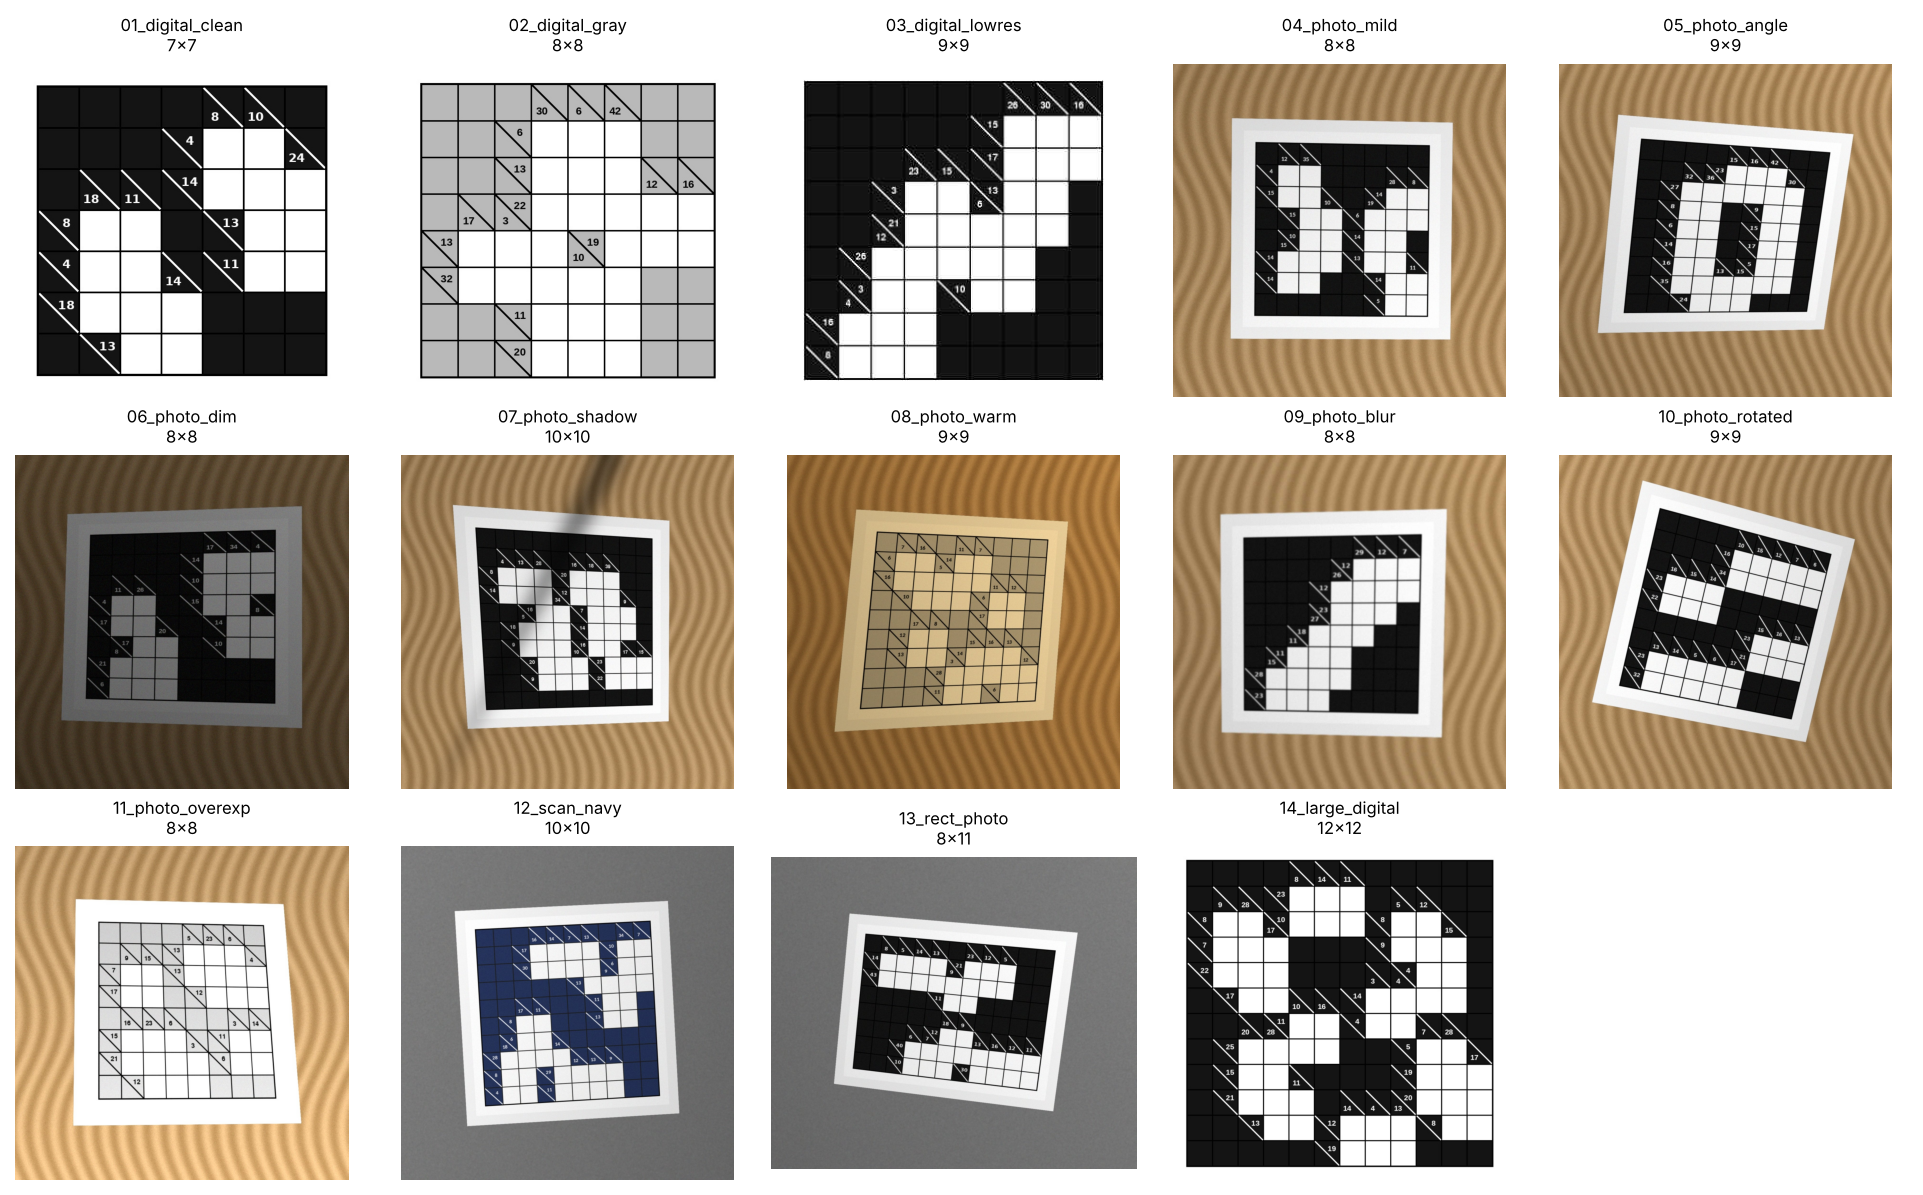
\includegraphics[width=\columnwidth]{dataset.png}
  \caption{Dataset de prueba: versiones digitales y fotografías con distintas condiciones de captura.}
  \label{fig:dataset}
\end{figure}

% ---------------------------------------------------------------------
\section{Fase 1: Visión Computacional e IA}
\subsection{Preprocesamiento y localización del tablero}
La imagen se reduce a un lado máximo de 1600\,px, se convierte a escala de grises y se suaviza con un filtro gaussiano $5\times5$. Se aplica un \textbf{umbral adaptativo gaussiano} (ventana $\approx$ 1/25 del lado, $C=7$) combinado con un umbral global de Otsu~\cite{otsu1979}. Sobre la imagen binaria se extraen todos los contornos (\texttt{RETR\_LIST}); cada uno se aproxima por su envolvente convexa y \texttt{approxPolyDP} con tolerancia creciente hasta obtener 4 vértices, y se exige que el contorno ocupe al menos el 80\,\% del cuadrilátero.

Una foto contiene además el borde de la hoja de papel, que también es un cuadrilátero grande. Para discriminarlo se usa conocimiento del dominio: en todo Kakuro la primera fila y la primera columna son bloques, por lo que la banda interior superior e izquierda del tablero es oscura respecto al nivel del papel, mientras que el margen de una hoja no lo es. Entre los candidatos con banda oscura se exige además una grilla periódica clara (Sec.~\ref{sec:grid}) y se elige el de mayor área (Fig.~\ref{fig:preproc}).

\begin{figure*}[t]
  \centering
  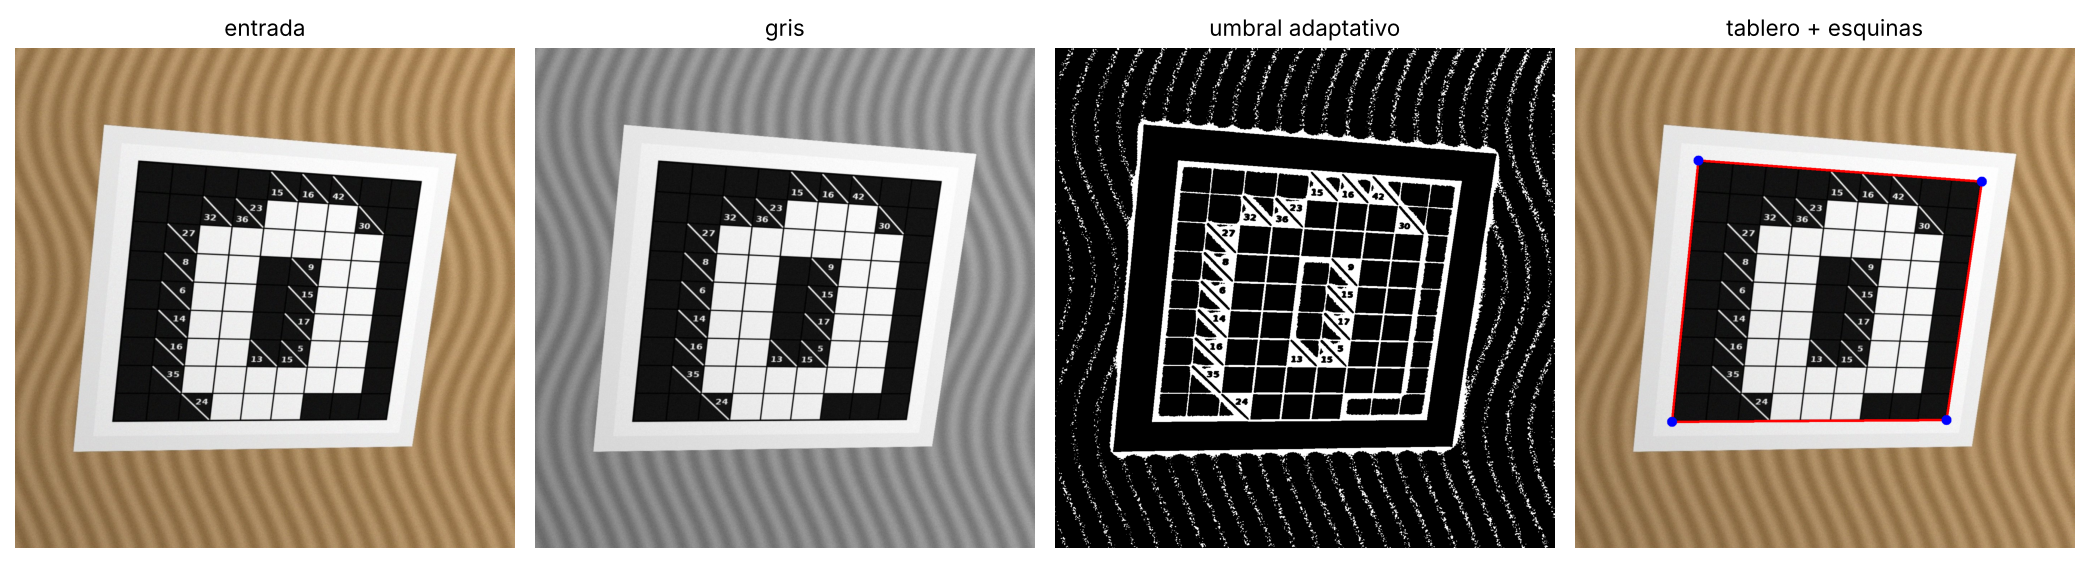
\includegraphics[width=\textwidth]{preproc.png}
  \caption{Preprocesamiento: imagen de entrada, escala de grises, umbral adaptativo y tablero localizado con sus esquinas.}
  \label{fig:preproc}
\end{figure*}

\subsection{Corrección de perspectiva y tamaño de la grilla}\label{sec:grid}
Con las esquinas ordenadas (TL, TR, BR, BL) se calcula la homografía $H$ al rectángulo de relación de aspecto estimada. Para estimar el número de columnas $n$ se proyecta la magnitud del gradiente de Sobel horizontal sobre el eje $x$, obteniendo el perfil $P_x$ de longitud $L$ (análogo para filas). Para cada $n\in[3,30]$ se evalúa
\begin{equation}
S(n)=\frac{1}{\sigma_P}\Big(\overline{P\!\left(\tfrac{kL}{n}\right)}_{k=1}^{n-1}-\overline{P\!\left(\tfrac{(k+\frac12)L}{n}\right)}_{k=0}^{n-1}\Big),
\end{equation}
es decir, el contraste entre las posiciones esperadas de las líneas y los centros de las celdas. Para $2n$ la mitad de las líneas hipotéticas caen en centros ($S$ bajo) y para $n/2$ los centros hipotéticos son líneas ($S\approx0$); los subarmónicos impares ($n/3$) sí puntúan alto, por lo que se toma $n_0=\arg\max S$ y luego el mayor múltiplo $kn_0$ con $S(kn_0)\ge0.5\,S(n_0)$. La Fig.~\ref{fig:grid} muestra el perfil y el puntaje. Finalmente se vuelve a rectificar a exactamente 96\,px por celda.

\begin{figure*}[t]
  \centering
  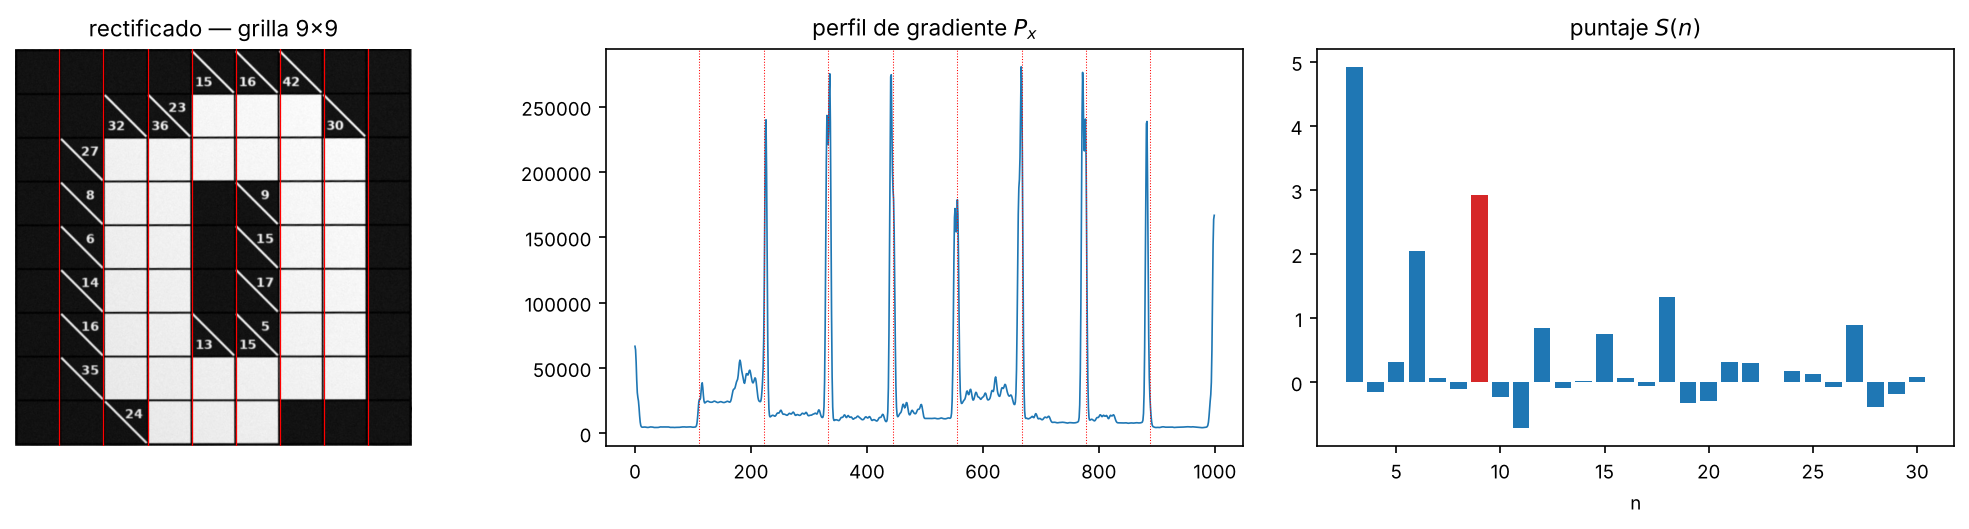
\includegraphics[width=\textwidth]{grid.png}
  \caption{Estimación del tamaño de grilla: tablero rectificado, perfil de gradiente $P_x$ y puntaje $S(n)$ (máximo en $n=9$).}
  \label{fig:grid}
\end{figure*}

\subsection{Clasificación de celdas}
Para cada celda se toma la mediana $m_{rc}$ de su 60\,\% central. Una umbralización directa falla cuando un bloque gris bien iluminado es más claro que una celda blanca en sombra, por lo que se ajusta un \textbf{modelo de iluminación cuadrático}
\begin{equation}
\log L(r,c)=\boldsymbol\beta^\top[1,\,r,\,c,\,r^2,\,c^2,\,rc]
\end{equation}
por mínimos cuadrados con muestras del papel en un anillo exterior al tablero (0.08--0.35 celdas fuera del borde) y, de forma iterativa, con las celdas ya clasificadas como blancas. La razón $\rho_{rc}=m_{rc}/L(r,c)$ se umbraliza con Otsu acotado a $[0.55,0.96]$ (Fig.~\ref{fig:cells}).

\begin{figure}[t]
  \centering
  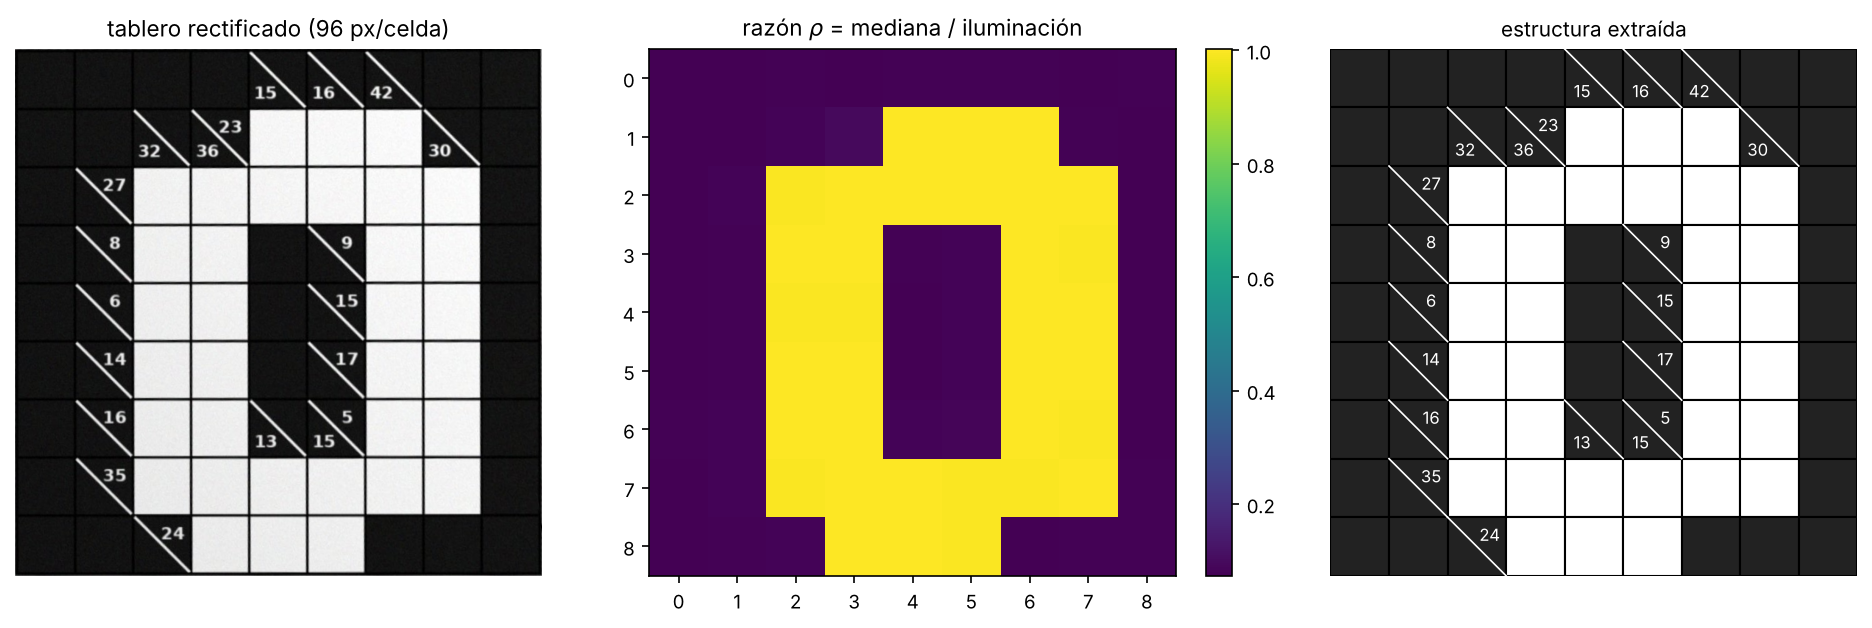
\includegraphics[width=\columnwidth]{cells.png}
  \caption{Tablero rectificado, razón $\rho$ normalizada por la iluminación y estructura extraída.}
  \label{fig:cells}
\end{figure}

\subsection{Lectura de las pistas}
Para cada bloque que inicia una suma se recorta la celda y:
\begin{enumerate}
  \item se detecta la \textbf{polaridad} (tinta clara sobre bloque oscuro o tinta oscura sobre bloque claro) comparando la mediana con los percentiles 2 y 98, y se binariza el contraste con Otsu;
  \item se \textbf{elimina la diagonal}: su desplazamiento real se estima como la moda de $y-x$ entre los píxeles de tinta cercanos a $y=x$, lo que tolera pequeños errores de rectificación, y se borra una banda de $\pm9\,\%$ de la celda; se descartan componentes con forma de línea (relleno $<18\,\%$);
  \item se extraen \textbf{componentes conexas} filtradas por altura y área; el centroide decide el triángulo ($x>y$: horizontal; si no, vertical) y los dígitos pegados (ancho $>1.15\times$ alto) se separan;
  \item cada dígito se centra en un cuadrado, se lleva a $28\times28$ y se describe con HOG (9 orientaciones, celdas $7\times7$, bloques $2\times2$)~\cite{dalal2005}, píxeles $14\times14$ y la relación de aspecto.
\end{enumerate}

\textbf{Red neuronal propia.} El clasificador es un perceptrón multicapa (256--128 neuronas ReLU, Adam, regularización $L_2$, parada temprana)~\cite{sklearn} entrenado con 24\,000 dígitos sintéticos renderizados en 12 tipografías libres con aumentos aleatorios: rotación $\pm7^\circ$, escala, erosión/dilatación, reducción de resolución, desenfoque y ruido. Su exactitud en validación sintética (dígitos aislados y fuertemente degradados) es \valacc\,\% (matriz de confusión en la Fig.~\ref{fig:ocr}).

\textbf{Corrección guiada por restricciones.} El clasificador entrega una distribución por dígito. Se usan dos propiedades del Kakuro: (i) una suma de $L$ celdas sólo admite pistas en $[\sum_{i=1}^{L}i,\ \sum_{i=10-L}^{9}i]$, así que se elige la lectura de mayor log-probabilidad (entre las 4 mejores clases de cada dígito) dentro de ese rango; (ii) la suma de todas las pistas horizontales es igual a la de las verticales (ambas suman todas las celdas blancas); si no se cumple, se sustituye la única pista cuya lectura alternativa restablece la igualdad con la menor pérdida de log-probabilidad.

\textbf{Comparación.} Como referencia se usa Tesseract~5 (motor LSTM)~\cite{smith2007} en modo de línea (\texttt{--psm 7}) con lista blanca de dígitos sobre la misma segmentación.

\begin{figure}[t]
  \centering
  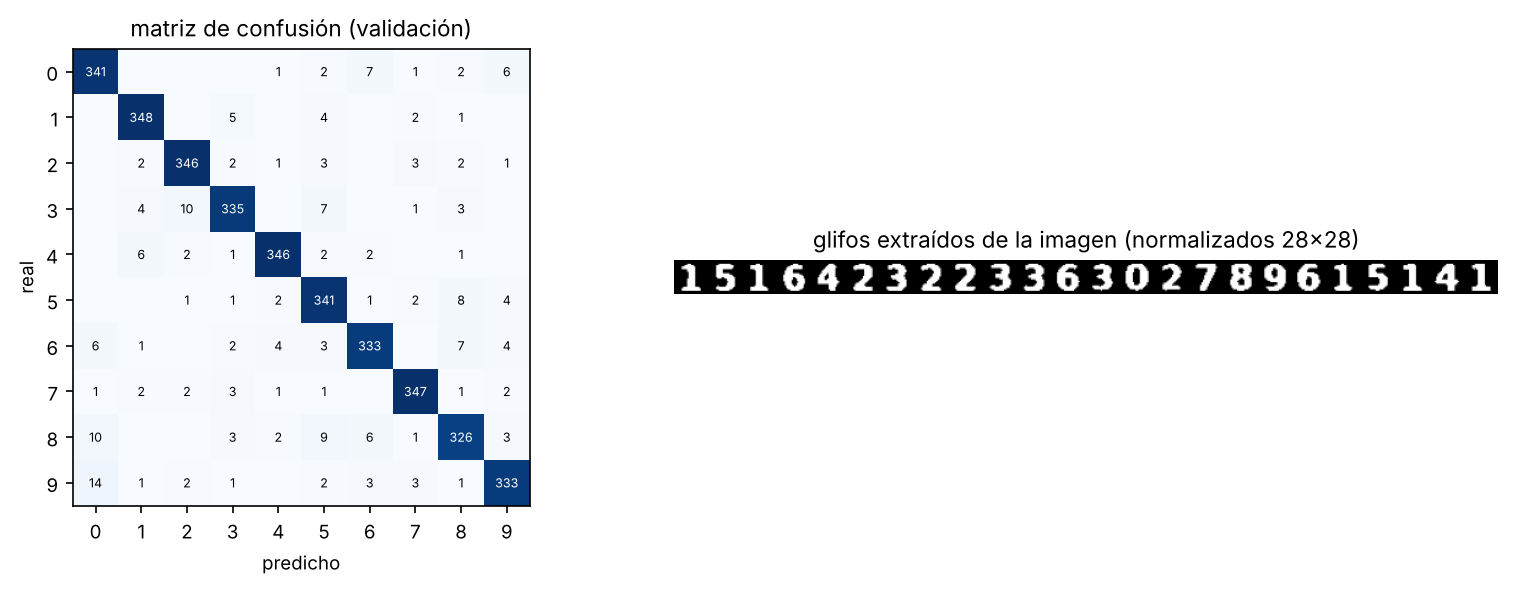
\includegraphics[width=\columnwidth]{ocr.png}
  \caption{Matriz de confusión del MLP en validación y glifos reales extraídos de una fotografía.}
  \label{fig:ocr}
\end{figure}

\subsection{Salida de la Fase 1}
El resultado es una estructura \texttt{Puzzle} serializable a JSON con \texttt{rows}, \texttt{cols} y las matrices \texttt{white}, \texttt{down} y \texttt{across}. Antes de pasar al solver se validan: longitudes de suma entre 2 y 9, pistas dentro de rango, toda celda blanca en una suma horizontal y una vertical, e igualdad de sumas globales.

% ---------------------------------------------------------------------
\section{Fase 2: Modelo de Constraint Programming}
\subsection{Formulación}
Sea $\mathcal{W}$ el conjunto de celdas blancas y $\mathcal{R}$ el conjunto de sumas; cada $R\in\mathcal{R}$ es una secuencia maximal de celdas blancas contiguas (horizontal o vertical) con pista $t_R$. Sea $\mathcal{C}(L,t)=\{S\subseteq\{1..9\}:|S|=L,\ \sum S=t\}$ el conjunto de combinaciones válidas.
\begin{itemize}
  \item \textbf{Variables:} $x_c$ para cada $c\in\mathcal{W}$.
  \item \textbf{Dominios:} $D(x_c)=\{1,\dots,9\}$ en el modelo base. En el modelo con filtrado:
  \begin{equation}
  D(x_c)=\bigcap_{R\ni c}\ \bigcup_{S\in\mathcal{C}(|R|,t_R)} S .
  \end{equation}
  \item \textbf{Restricciones}, para todo $R\in\mathcal{R}$:
  \begin{align}
  &\texttt{AllDifferent}\,(x_c : c\in R) \label{eq:ad}\\
  &\textstyle\sum_{c\in R} x_c = t_R \label{eq:sum}\\
  &\texttt{Table}\big((x_c)_{c\in R},\ T_R\big)\quad\text{si } |R|\le4, \label{eq:table}\\
  &\quad T_R=\{\pi(S):S\in\mathcal{C}(|R|,t_R),\ \pi\in\Pi_{|R|}\}\nonumber
  \end{align}
  \item \textbf{Objetivo:} ninguno (problema de satisfacción). Se verifica además la unicidad de la solución.
\end{itemize}
El modelo es \textbf{parametrizado}: se construye recorriendo las sumas de cualquier \texttt{Puzzle} producido por la visión. Se implementan tres variantes en OR-Tools CP-SAT~\cite{ortools}: \texttt{global} (\ref{eq:ad})--(\ref{eq:sum}); \texttt{global\_dom}, que añade el filtrado de dominios y (\ref{eq:table}); y \texttt{reified}, descrita en la Sec.~\ref{sec:reif}. La tabla se limita a $|R|\le4$ porque su tamaño es $|\mathcal{C}|\cdot|R|!$ tuplas (como mucho 24 por combinación en ese caso), mientras que para $|R|=9$ crecería a $9!$.

\begin{lstlisting}[caption={Núcleo del modelo en CP-SAT (\texttt{kakuro/solver.py}).}]
for run in puzzle.runs():
    xs = [x[c] for c in run.cells]
    m.Add(sum(xs) == run.total)          # Sum
    m.AddAllDifferent(xs)                 # AllDifferent
    if len(run) <= 4:                     # Table
        m.AddAllowedAssignments(xs, [p for s in
            combos(len(run), run.total) for p in permutations(s)])
\end{lstlisting}

\subsection{Restricciones globales y propagación}
\texttt{AllDifferent} y \texttt{Sum} sobre la misma suma interactúan: su conjunción equivale a que el \emph{conjunto} de valores pertenezca a $\mathcal{C}(L,t)$. Propagarlas por separado pierde poda; por ejemplo, para $L=2$, $t=16$ los cotas permiten $\{7,8,9\}$, pero sólo $\{7,9\}$ es válida. Por ello, además de CP-SAT, se implementó un motor propio (\texttt{kakuro/cp\_engine.py}) con un propagador que alcanza \textbf{consistencia de arco generalizada} (GAC) sobre la conjunción, mediante programación dinámica sobre subconjuntos de dígitos (Algoritmo~\ref{alg:gac}): como el conjunto de dígitos usados determina la suma, basta recorrer las máscaras alcanzables hacia adelante y hacia atrás, con costo $O(L\cdot\binom{9}{\lfloor 9/2\rfloor}\cdot 9)$ por invocación. La búsqueda es DFS con la heurística MRV (dominio mínimo) y propagación hasta punto fijo con una cola de restricciones (estilo AC-3). Como contraste, el nivel \emph{cotas} sólo elimina valores ya asignados y razona sobre la suma mínima y máxima.

\begin{algorithm}[t]
\caption{GAC para $\texttt{AllDifferent}(x_{1..L})\wedge\sum x_i=t$}\label{alg:gac}
\begin{algorithmic}[1]
\Require dominios $D_1..D_L$ (máscaras de bits), pista $t$
\State $F_0\gets\{\emptyset\}$
\For{$i=1..L$} \Comment{hacia adelante}
  \State $F_i\gets\{M\cup\{d\}: M\in F_{i-1},\ d\in D_i\setminus M\}$
\EndFor
\State $B_L\gets\{M\in F_L:\ \sum M=t\}$; \textbf{si} $B_L=\emptyset$ \textbf{fallar}
\For{$i=L..1$} \Comment{hacia atrás}
  \State $D'_i\gets\{d\in D_i:\exists M\in F_{i-1},\ d\notin M,\ M\cup\{d\}\in B_i\}$
  \State $B_{i-1}\gets\{M\in F_{i-1}:\exists d\in D_i\setminus M,\ M\cup\{d\}\in B_i\}$
  \State \textbf{si} $D'_i=\emptyset$ \textbf{fallar}
\EndFor
\Ensure dominios podados $D'_1..D'_L$
\end{algorithmic}
\end{algorithm}

La Tabla~\ref{tab:root} cuantifica la poda \emph{antes de buscar}: el espacio inicial de hasta $10^{55}$ asignaciones se reduce a $10^{9}$--$10^{30}$ con cotas, mientras que con GAC 9 de los 14 puzzles quedan completamente resueltos en la raíz y en el resto se fija entre 26\,\% y 78\,\% de las celdas.

\begin{table*}[t]
\centering
\caption{Propagación en la raíz: tamaño del espacio de búsqueda ($\log_{10}\prod|D(x_c)|$) antes y después de propagar.}
\label{tab:root}
\small
\begin{tabular}{lrrrrr}
\toprule
imagen & celdas & log10 espacio inicial & log10 tras cotas & log10 tras GAC & fijadas por GAC (\%) \\
\midrule
01 digital clean & 18 & 17.2 & 8.6 & 0.0 & 100.0 \\
02 digital gray & 28 & 26.7 & 18.9 & 0.0 & 100.0 \\
03 digital lowres & 30 & 28.6 & 19.7 & 6.5 & 40.0 \\
04 photo mild & 26 & 24.8 & 11.7 & 0.0 & 100.0 \\
05 photo angle & 34 & 32.4 & 23.8 & 13.6 & 26.5 \\
06 photo dim & 24 & 22.9 & 12.5 & 5.5 & 50.0 \\
07 photo shadow & 40 & 38.2 & 26.1 & 0.0 & 100.0 \\
08 photo warm & 32 & 30.5 & 13.9 & 0.0 & 100.0 \\
09 photo blur & 23 & 21.9 & 18.0 & 0.0 & 100.0 \\
10 photo rotated & 32 & 30.5 & 19.9 & 0.0 & 100.0 \\
11 photo overexp & 28 & 26.7 & 10.7 & 0.0 & 100.0 \\
12 scan navy & 40 & 38.2 & 23.7 & 6.0 & 60.0 \\
13 rect photo & 34 & 32.4 & 22.2 & 0.0 & 100.0 \\
14 large digital & 58 & 55.3 & 29.7 & 6.6 & 77.6 \\
\bottomrule
\end{tabular}

\end{table*}

\subsection{Restricciones reificadas}\label{sec:reif}
El modelo principal \textbf{no requiere reificación}: todas las reglas del Kakuro son incondicionales (toda suma debe ser exacta y sin repetidos), por lo que se expresan directamente con restricciones globales, que además propagan más que su descomposición booleana. La reificación se usa donde aporta:
\begin{itemize}
  \item \textbf{Prueba de unicidad.} Tras obtener una solución $s$, se añaden literales $d_c$ con la semi-reificación $d_c\Rightarrow x_c\neq s_c$ (\texttt{OnlyEnforceIf}) y la cláusula $\bigvee_{c} d_c$. Si el modelo resultante es infactible, la solución es única. Así se validó cada instancia del dataset y del benchmark.
  \item \textbf{Modelo \texttt{reified}} (comparación): codificación \emph{one-hot} $b_{c,d}\Leftrightarrow(x_c=d)$, $\texttt{ExactlyOne}_d(b_{c,d})$ por celda y $\texttt{AtMostOne}_{c\in R}(b_{c,d})$ por suma y dígito en lugar de \texttt{AllDifferent}. Requiere $9|\mathcal{W}|$ variables booleanas adicionales y permite medir el costo de sustituir la restricción global por su descomposición reificada.
\end{itemize}

\subsection{Análisis de complejidad}
El problema de decisión es NP-completo~\cite{seta2002,ruepp2010}, por lo que el peor caso es exponencial; el espacio ingenuo es $9^{|\mathcal{W}|}$. La construcción del modelo es lineal en el tamaño de la instancia: $|\mathcal{W}|$ variables y $2|\mathcal{R}|$ restricciones (más $|\mathcal{R}_{\le4}|$ tablas con $O(|\mathcal{C}|\cdot 24)$ tuplas). En la práctica, la propagación fuerte de las restricciones globales hace que los puzzles bien planteados (solución única) se resuelvan con muy poca búsqueda.

Para medir tiempos se generaron 18 instancias con solución única de $6\times6$ a $16\times16$ (12--103 celdas blancas). La Tabla~\ref{tab:bench} y la Fig.~\ref{fig:bench} reportan, con el \solverbackend, el tiempo de obtener la solución \emph{y} demostrar su unicidad (mediana de 3 ejecuciones) y el número de nodos. Con propagación por cotas el número de nodos crece rápidamente con el tamaño (hasta 1408 nodos y cerca de 0.2\,s en $14\times14$), mientras que con filtrado de dominios y GAC se mantiene en 1--35 nodos y por debajo de 3\,ms incluso en $16\times16$. El tiempo del solver es despreciable frente a la fase de visión.

\begin{table*}[t]
\centering
\caption{Tiempo medio (ms, solución + prueba de unicidad) y nodos explorados por tamaño de tablero.}
\label{tab:bench}
\small
\begin{tabular}{rrrrrr}
\toprule
n & celdas & native/global ms & native/global-dom ms & native/global nodos & native/global-dom nodos \\
\midrule
6 & 14.00 & 0.43 & 0.03 & 5.00 & 1.00 \\
8 & 23.33 & 1.85 & 0.07 & 12.33 & 1.00 \\
10 & 38.33 & 2.12 & 0.10 & 15.00 & 1.00 \\
12 & 60.67 & 13.94 & 0.38 & 58.00 & 4.00 \\
14 & 80.00 & 97.71 & 0.98 & 639.00 & 5.00 \\
16 & 102.67 & 21.94 & 0.92 & 143.67 & 16.00 \\
\bottomrule
\end{tabular}

\end{table*}

\begin{figure}[t]
  \centering
  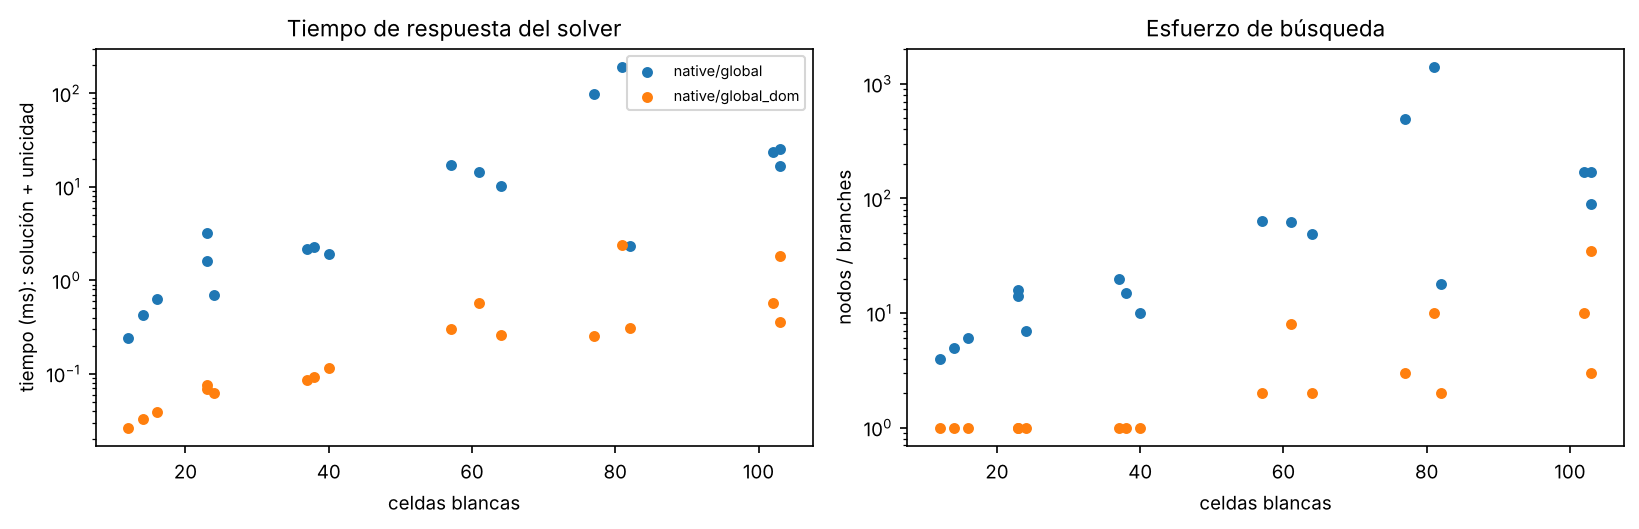
\includegraphics[width=\columnwidth]{bench.png}
  \caption{Tiempo de respuesta y esfuerzo de búsqueda del solver frente al número de celdas blancas (escala logarítmica).}
  \label{fig:bench}
\end{figure}

% ---------------------------------------------------------------------
\begin{figure*}[t]
  \centering
  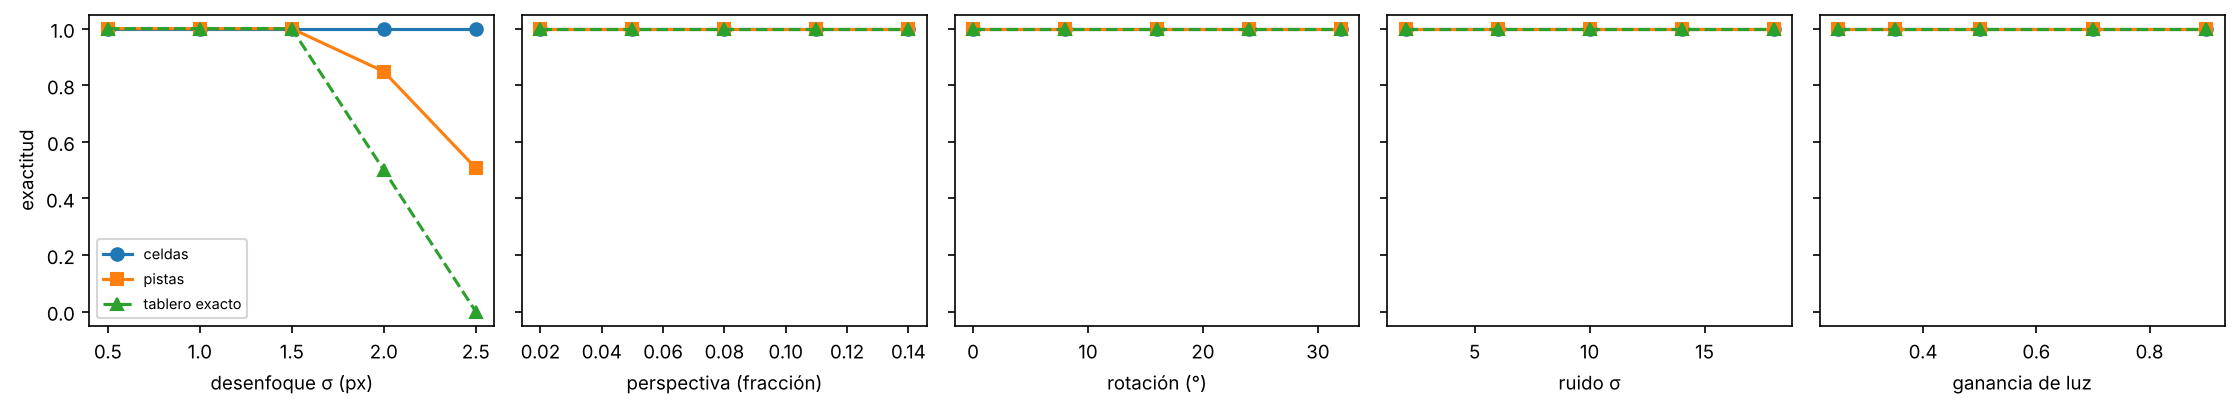
\includegraphics[width=\textwidth]{robustness.png}
  \caption{Barrido de robustez: exactitud de celdas, pistas y tableros exactos frente a cada degradación (4 imágenes por nivel).}
  \label{fig:rob}
\end{figure*}

\section{Fase 3: Integración y visualización}
La función \texttt{solve\_image} encadena las tres fases sin intervención manual: la estructura \texttt{Puzzle} producida por la visión es la entrada directa del constructor del modelo CP. La solución se dibuja sobre el tablero rectificado y se re-proyecta a la foto original con $H^{-1}$, de modo que los dígitos aparecen en perspectiva sobre la hoja (Fig.~\ref{fig:overlay}); además se genera una grilla limpia con matplotlib. El sistema también se ofrece como comando: \texttt{python -m kakuro.pipeline foto.jpg --out solucion.jpg}.

\begin{figure}[t]
  \centering
  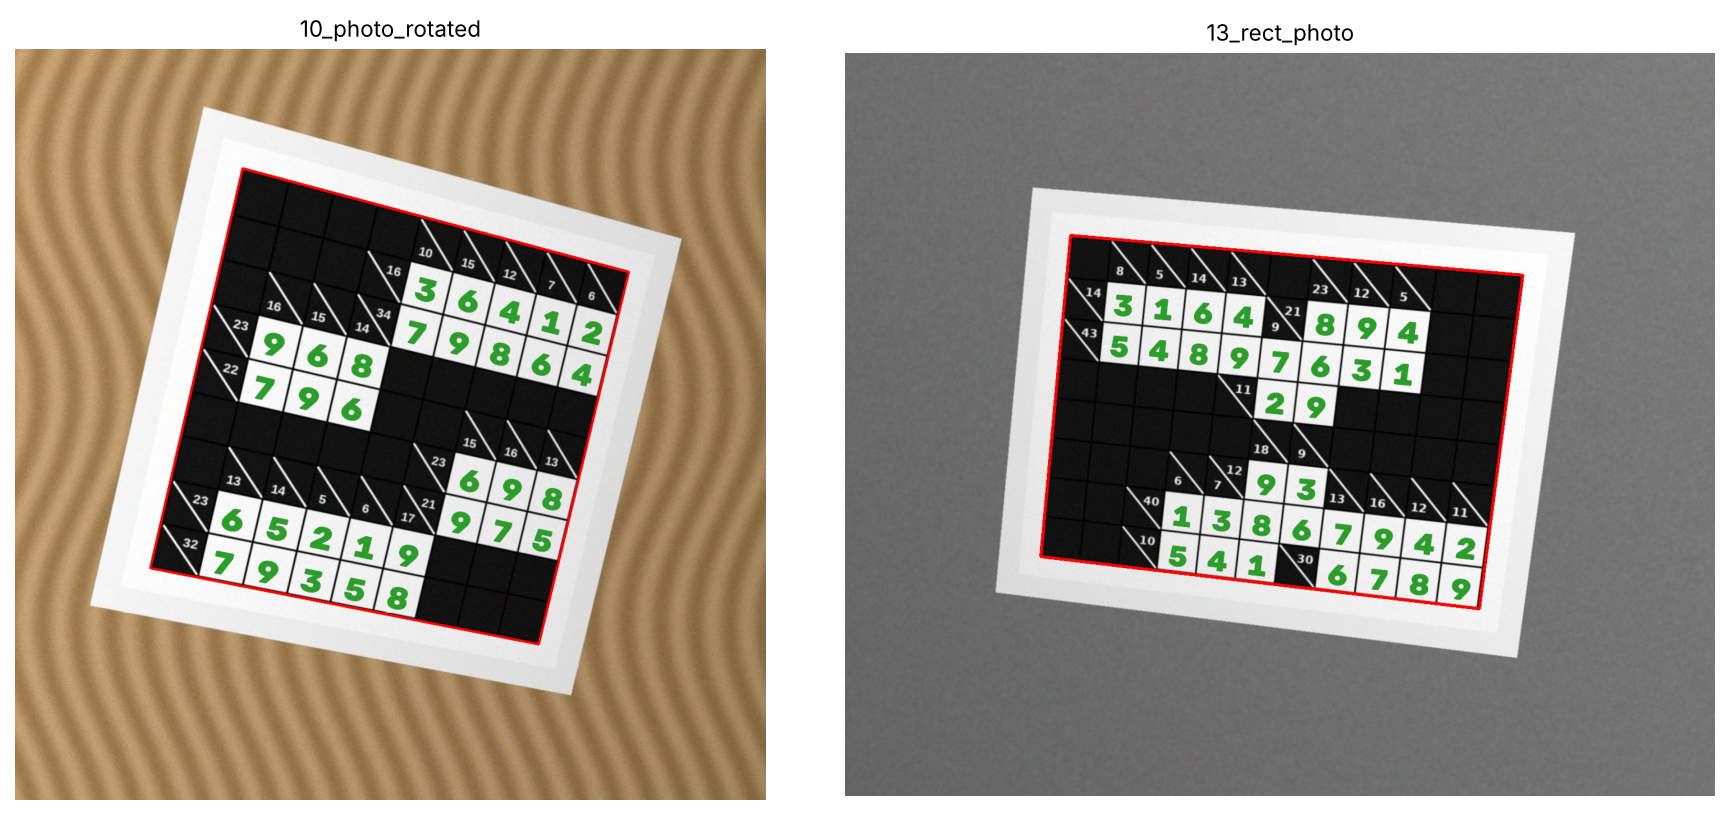
\includegraphics[width=\columnwidth]{overlay_examples.png}
  \caption{Solución re-proyectada sobre la imagen original (foto rotada y tablero rectangular).}
  \label{fig:overlay}
\end{figure}

% ---------------------------------------------------------------------
\section{Resultados experimentales}
\subsection{Precisión de la visión}
La Tabla~\ref{tab:vision} resume las métricas sobre el dataset y la Tabla~\ref{tab:perimg} el detalle por imagen. La grilla y la clasificación blanca/negra son correctas en el 100\,\% de los casos (1\,125 celdas). El MLP lee correctamente 313 de 314 pistas sin corrección (99.7\,\%): el único error (39 leído como 30 bajo una sombra) es reparado por el invariante global de sumas, de modo que el sistema completo alcanza 314/314 y resuelve los 14 puzzles. Tesseract, con la misma segmentación, lee el 92.4\,\% de las pistas y sólo 4 tableros quedan exactos, pues sus errores se concentran en dígitos pequeños, invertidos o degradados (baja resolución, desenfoque, escaneo azul); ver Fig.~\ref{fig:ocrcmp}.

\begin{table}[t]
\centering
\caption{Métricas de la Fase 1 sobre las 14 imágenes.}
\label{tab:vision}
\small
\begin{tabular}{lrrr}
\toprule
métrica & MLP+corr. & MLP & Tesseract \\
\midrule
grilla correcta & 1.000 & 1.000 & 1.000 \\
exactitud celdas & 1.000 & 1.000 & 1.000 \\
exactitud pistas & 1.000 & 0.997 & 0.924 \\
tableros exactos & 1.000 & 0.929 & 0.286 \\
resueltos correctamente & 1.000 & 0.929 & 0.286 \\
t. visión medio (s) & 0.112 & 0.111 & 2.307 \\
\bottomrule
\end{tabular}

\end{table}

\begin{table}[t]
\centering
\caption{Resultados por imagen: exactitud de celdas y pistas correctas por método.}
\label{tab:perimg}
\scriptsize
\setlength{\tabcolsep}{3pt}
\begin{tabular}{lrrrrrl}
\toprule
imagen & celdas & pistas & MLP+corr. & MLP & Tesseract & resuelto \\
\midrule
01 digital clean & 1.000 & 14 & 14 & 14 & 14 & sí \\
02 digital gray & 1.000 & 16 & 16 & 16 & 16 & sí \\
03 digital lowres & 1.000 & 18 & 18 & 18 & 15 & sí \\
04 photo mild & 1.000 & 20 & 20 & 20 & 18 & sí \\
05 photo angle & 1.000 & 20 & 20 & 20 & 20 & sí \\
06 photo dim & 1.000 & 18 & 18 & 18 & 16 & sí \\
07 photo shadow & 1.000 & 26 & 26 & 25 & 24 & sí \\
08 photo warm & 1.000 & 26 & 26 & 26 & 23 & sí \\
09 photo blur & 1.000 & 14 & 14 & 14 & 10 & sí \\
10 photo rotated & 1.000 & 24 & 24 & 24 & 23 & sí \\
11 photo overexp & 1.000 & 22 & 22 & 22 & 21 & sí \\
12 scan navy & 1.000 & 28 & 28 & 28 & 24 & sí \\
13 rect photo & 1.000 & 24 & 24 & 24 & 24 & sí \\
14 large digital & 1.000 & 44 & 44 & 44 & 42 & sí \\
\bottomrule
\end{tabular}

\end{table}

\begin{figure}[t]
  \centering
  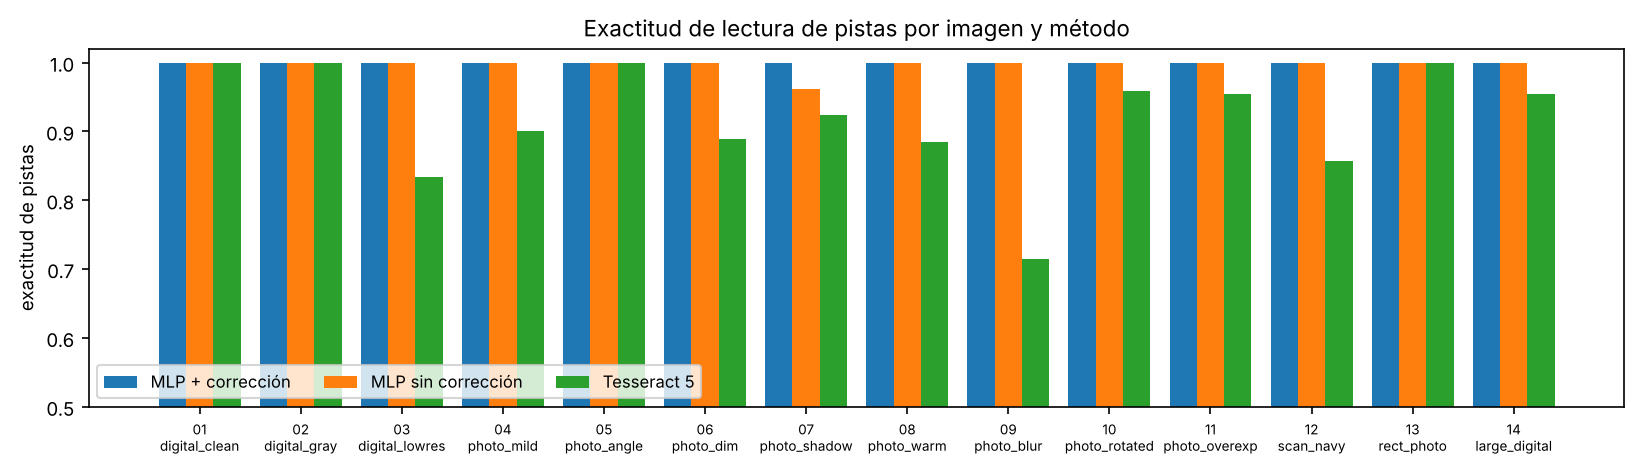
\includegraphics[width=\columnwidth]{ocr_compare.png}
  \caption{Exactitud de lectura de pistas por imagen: MLP con y sin corrección frente a Tesseract~5.}
  \label{fig:ocrcmp}
\end{figure}

\subsection{Robustez}
Para estimar los límites del sistema se generaron 100 imágenes adicionales con puzzles, estilos y tipografías aleatorios, degradando un factor a la vez (Fig.~\ref{fig:rob}). El sistema es estable frente a perspectiva (hasta 14\,\% del lado), rotación (hasta $32^\circ$), ruido ($\sigma=18$) y luz baja (ganancia 0.25). El factor limitante es el desenfoque: con $\sigma\ge2$\,px la exactitud de pistas cae a 85\,\% y con $\sigma=2.5$\,px a 51\,\%, porque los dígitos de dos cifras se funden; la grilla y las celdas siguen siendo correctas.



\subsection{Tiempos de respuesta}
En CPU, el tiempo medio por imagen es de 0.16\,s: localización del tablero 43\,ms, grilla 10\,ms, celdas 16\,ms, OCR 45\,ms y solver 0.2\,ms (incluida la prueba de unicidad). Tesseract eleva el tiempo de visión a 2.3\,s por imagen.

% ---------------------------------------------------------------------
\section{Discusión y limitaciones}
La validación con conocimiento del dominio (bandas oscuras, periodicidad, rangos de suma e invariante global) es lo que hace robusto al sistema: cada etapa descarta hipótesis inconsistentes con las reglas del Kakuro. Las principales limitaciones son: (i) el dataset de evaluación es sintético, aunque las tipografías difieren de las de entrenamiento y las degradaciones simulan una cámara; conviene ampliarlo con fotografías reales de periódicos y revistas, que el código admite sin cambios; (ii) se asume que el tablero se ve completo y con margen, y que las pistas siguen la convención de diagonal estándar; (iii) el desenfoque fuerte degrada el OCR, lo que podría mitigarse con una CNN entrenada con más desenfoque o con una segmentación por cuencas de los dígitos pegados.

% ---------------------------------------------------------------------
\section{Conclusiones}
Se construyó un sistema extremo a extremo que lee un Kakuro desde una imagen y lo resuelve con CP sin intervención manual. La combinación de visión clásica, una red neuronal propia y correcciones basadas en las restricciones del puzzle logró 100\,\% de exactitud en grilla, celdas y pistas en el dataset, superando a Tesseract en lectura de pistas (100\,\% frente a 92.4\,\%). El modelo CP parametrizado con \texttt{AllDifferent}, \texttt{Sum} y \texttt{Table} resuelve y demuestra la unicidad en milisegundos, y el propagador GAC de la conjunción reduce la búsqueda a unos pocos nodos incluso en tableros de $16\times16$.

% ---------------------------------------------------------------------
\begin{thebibliography}{99}
\bibitem{wiki_kakuro} ``Kakuro,'' \emph{Wikipedia}. [En línea]. Disponible: \url{https://en.wikipedia.org/wiki/Kakuro}
\bibitem{seta2002} T. Seta, ``The complexities of puzzles, cross sum and their another solution problems (ASP),'' Tesis de licenciatura, Univ. de Tokio, 2002.
\bibitem{ruepp2010} O. Ruepp y M. Holzer, ``The computational complexity of the Kakuro puzzle, revisited,'' en \emph{Fun with Algorithms (FUN)}, LNCS 6099, Springer, 2010, pp.~319--330.
\bibitem{simonis2005} H. Simonis, ``Sudoku as a constraint problem,'' en \emph{CP Workshop on Modeling and Reformulating Constraint Satisfaction Problems}, 2005, pp.~13--27.
\bibitem{regin1994} J.-C. Régin, ``A filtering algorithm for constraints of difference in CSPs,'' en \emph{Proc. AAAI}, 1994, pp.~362--367.
\bibitem{rossi2006} F. Rossi, P. van Beek y T. Walsh (eds.), \emph{Handbook of Constraint Programming}. Elsevier, 2006.
\bibitem{ortools} L. Perron y F. Didier, ``CP-SAT,'' Google OR-Tools, 2024. [En línea]. Disponible: \url{https://developers.google.com/optimization}
\bibitem{otsu1979} N. Otsu, ``A threshold selection method from gray-level histograms,'' \emph{IEEE Trans. Syst., Man, Cybern.}, vol.~9, no.~1, pp.~62--66, 1979.
\bibitem{opencv} G. Bradski, ``The OpenCV library,'' \emph{Dr. Dobb's Journal of Software Tools}, 2000.
\bibitem{smith2007} R. Smith, ``An overview of the Tesseract OCR engine,'' en \emph{Proc. ICDAR}, 2007, pp.~629--633.
\bibitem{dalal2005} N. Dalal y B. Triggs, ``Histograms of oriented gradients for human detection,'' en \emph{Proc. CVPR}, 2005, pp.~886--893.
\bibitem{sklearn} F. Pedregosa \emph{et al.}, ``Scikit-learn: Machine learning in Python,'' \emph{J. Mach. Learn. Res.}, vol.~12, pp.~2825--2830, 2011.
\end{thebibliography}

\end{document}
